\documentclass[conference]{IEEEtran}
\IEEEoverridecommandlockouts
% The preceding line is only needed to identify funding in the first footnote. If that is unneeded, please comment it out.
\usepackage{cite}
\usepackage{amsmath,amssymb,amsfonts}
\usepackage{algorithmic}
\usepackage{graphicx}
\usepackage{textcomp}
\usepackage{xcolor}
%\usepackage[dvipdfmx]{}
\def\BibTeX{{\rm B\kern-.05em{\sc i\kern-.025em b}\kern-.08em
    T\kern-.1667em\lower.7ex\hbox{E}\kern-.125emX}}

\newcommand{\SSID}{S_{A_{target}}}
\newcommand{\tarMAC}{M_{A_{target}}}
\newcommand{\userMAC}{M_{user_device}}
\newcommand{\inputAP}{A_{input}}
\newcommand{\tarAP}{A_{target}}
\begin{document}

\title{Conference Paper Title*\\
{\footnotesize \textsuperscript{*}Note: Sub-titles are not captured in Xplore and
should not be used}
\thanks{identify applicable funding agency here. If none, delete this.}
}

\author{\IEEEauthorblockN{1\textsuperscript{st} Given Name Surname}
\IEEEauthorblockA{\textit{dept. name of organization (of Aff.)} \\
\textit{name of organization (of Aff.)}\\
City, Country \\
email address or ORCID}
\and
\IEEEauthorblockN{2\textsuperscript{nd} Given Name Surname}
\IEEEauthorblockA{\textit{dept. name of organization (of Aff.)} \\
\textit{name of organization (of Aff.)}\\
City, Country \\
email address or ORCID}
\and
\IEEEauthorblockN{3\textsuperscript{rd} Given Name Surname}
\IEEEauthorblockA{\textit{dept. name of organization (of Aff.)} \\
\textit{name of organization (of Aff.)}\\
City, Country \\
email address or ORCID}
\and

}

\maketitle

\begin{abstract}
Detecting a rougue AP (RAP) in Wi-Fi network is imperative.
The existing schemes are divided into network administrator side detections and user side detections.
The former is inapplicable to the free Wi-Fi network due to the cost problem.
Although the latter can be introduced every Wi-Fi network, its detection performances depend on the real environment or performance of a RAP.
Thus, it is necessary to design the scheme which is independent of such factors.
In this paper, we propose \title.
Since the RAP is established between a user device and legitimate AP (LAP), in attack case, there exists two APs on the path.
On the basis of this idea, the proposed scheme reveal the connected AP as a RAP by searching another AP on the path besides the connected AP.
In order to finding a LAP out, the proposed scheme observes ARP procedure to detect its MAC address.
By setting MAC address of a user device to that of LAP which is on the same path, ARP reply packets from a gateway does not sent to the user device as in usual.
As aresult, the proposed scheme achieves an accuracy of 96.5\%.
True positive rate and false positive rate are 31.0\% higher and 9.0\% lower than the previous scheme even in unstable traffic environment. 
Furthermore, by extending the observation time of ARP procedure, we realize an accuracy of 100.0\% without any error.
The proposed scheme can detect RAPs accurately even in a real environment where the prevous scheme cannnot.
\end{abstract}

\begin{IEEEkeywords}
component, formatting, style, styling, insert
\end{IEEEkeywords}

\section{INTRODUCTION}
With the rapid development of wireless communication techniques, Wi-Fi as the most commonly used Internet access technology is deployed and keeps spreading all over the world to everywhere of our daily life, such as shopping malls, restaurants, public transit systems and so on.
While the free access to Wi-Fi network attarcts a large number of users, it also allows an adversary to launch attacks to users just by setting up a rogue AP (RAP) in the network.
An Evil Twin Attack is one of the attack where a RAP is established between a user device and the Internet as man-in-the-middle.
The RAP clones the service set identifier (SSID) and or even MAC address of a legitimate AP provided by a public facility, which is the reason why it is called "evil twin attack".
By acting as man-in-the-middle and observing relayed packets between a user device and LAP, an adversary can eavesdrop on the exchange of sensitive information such as identity credentials, passwords, and bank account.
In addition, an adversary can also mount an acctive attack by leading a user to phishing websites or infecting a user device with malicious softwares.
Since, our wireless devices connect automatically to an AP which has the strongest received signal strength indication (RSSI) of all APs which have same SSID and moreover they are provided Internet services as usual, an adversary can succed an attack without being noticed by a user.
Thus, the detection of the RAPs is urgent demand.

The attack is divided into two models based on how a RAP provide the Internet service to user device.
A model where a RAP use mobile communication can be detected easily with Internet Services Provider (ISP) names or Global IP addresses\cite{rtt}.
We focus on another model where a RAP uses same gateway with LAPs in the network by connecting with one of it since it cannot be detected by existing schemes.
During an early stage, the RAP detection is network administrator side detection based on whitelist-based mechanisms\cite{prapd}\cite{clockskew }.
However, those solutions are inapplicable to Wi-Fi hotspots since administrators have little motivation to guarantee no attacks by setting up additional devices in their infrastructures.
In order to realize applicable detection, the user side detections based on communication features have been proposed\cite{rtt}\cite{previous}.
Nevertheless, these existing approachs depend on an attack model or environment.

In order to realize the user side detection which is independent of other factors, in this paper, we propose \title.
The main idea of our scheme is that there exist two APs, namely the RAP and a LAP, on the same path from a user device to a gateway.
Therefore, in an attack scenario, besides the connected RAP, a LAP exists inevitably on the other side of the RAP due to a man-in-the-middle.
On the basis of this idea, the proposed scheme reveals the connected AP as RAP by finding MAC address of such LAP from obtainable beacon frames by a user device.
However, a user device cannnot distinguish the path of LAPs only by acquiring candidate MAC addresses.
Thus, we focus on the phenomenon that a user device connot receive Address Resolution Protocol (ARP) reply packets from a gateway in the situation where there exist duplicate MAC addresses on the same path.
The proposed scheme intentionally creates such situation by setting the MAC address of a user device to the candidate MAC addresses and finds out the one that a LAP on the same path has.
By doing this, the proposed scheme can reveal the connected AP as RAP in a attack scenario.
The contributions of our scheme are as follows:
\begin{enumerate}
    \renewcommand{\labelenumi}{\arabic{enumi}).}
    \item To the best of our knowledge, the proposed scheme is the first one which does not require features of the RAP. By taking advantage of the feature of a LAP, the proposed detection does not allow an adversary to avoid it by manipulating features of a RAP.
    \item The proposed scheme achieves accurate detection performance without any error even in a real environment. It is independent of other factors unlike existing works.
\end{enumerate}
The rest of this paper is constructed as follows: Related works are described in Section \ref{sec:2}.
The attack model, previous scheme and its shortcoming are intriduced in Section \ref{sec:3}.
The proposed scheme is explained in Section \ref{sec:4}.
Various evaluation results are shown in Section \ref{sec:5}.
Finally, the conclusions of this paper are presented in Section \ref{sec:6}.

\section{RELATED WORKS}\label{sec:2}
Rogue AP (RAP) detection methods are mainly classified into two categories: network administrator side detections and user side detections.
Network administrator side detections focus on the physical features such as Received Signal Strength Indication (RSSI) and clock skew which cannot be spoofed by an adversary.
RAP can be detected by comparing with the physical features of it with those in the predefined whitelist with equipments such as traffic sensors in each Wi-Fi network.

Wu et al. \cite{prapd} pay attention to the RSSI which is hard to be forged arbitrarily and highly correlated to the transmitter's location and power.
For each LAP in a network, RSSI, which is measured by additional costly devices, is registered as the information in whitelist beforehand.
By using RSSI, even if the MAC address of an AP is identical to that in the whitelist, that scheme can disclose that it is a RAP with spoofed MAC address set by an adversary at different location.
However, that scheme is hard to detect RAP which is located near the LAP because RSSI is not as exact as it can indicate a small difference of the nearby location. 
%Although it is useful as a supplementary feature, using only RSSI is insufficient to detect a RAP with high accuracy.

In order to detect in more detail, Lanze et al. \cite{clockskew} focus on clock skew as a device fingerprinting based purely on physical properties.
Clock skew is an unvoidable physical phenomenon that causes crystal oscillator based clocks to run with minuscule yet measurable deviations in speed.
However, these network administrator side detections are inapplicable to Wi-Fi hotspots because they have to setup additional sensors or install detection software in their infrastructure to prevent attacks besides providing free Internet service.
Thus, the detection schemes that require no equipment of additional devices by a network administrator are desired.

Meanwhile, user side detections do not need to introduce additional devices to a Wi-Fi hotspot. 
They focus on differences in the transmission characteristics caused by the extra hop to a RAP on the path between a LAP and user device. 
Compared with legitimate networks, extra hop results in several measurable changes in transmission characteristics such as Round Trip Time (RTT) and channel used between a user device and DNS server.

Mustafa et al. \cite{rtt} differentiate RAPs from LAPs by measuring the RTT between the user device and the DNS server through different target APs (RAPs or LAPs).
Because there exists the extra hop caused by the RAP on the path, RTT is longer in comparison to the case where a user directly connects to the LAP.
Although that scheme which leverages the packet delay are useful only for the case where the adversary sets RAP up on the laptop, Jang et al. \cite{previous} reveal the fact that the computational power of the software bridging mainly accounts for the packet delay.
Thus, the adversary can evade the packet delay based detection by utilizing hardware-based RAPs having little bridging delay unlike software-based RAPs.

In order to detect both types of RAPs, namely, software-based and hardware-based ones, \cite{previous} focuses on two communication channels utilized by a RAP between a user device and LAP.
Whereas a RAP intervene between a user device and LAP, two distinct channels are used to reduce communication delay caused by channel interference each other.
For example, it is assumed that channel 1 is used as the channel between a user device and a RAP, and channel 6 is that between a RAP and a LAP.
That scheme detects RAP by finding out the presence of these two channels with the throughput of the transmission from the user device to the DNS server.
That scheme is the most robust user side detection which is independent of the performance of the RAP because it is the countermeasure against a reasonable attack model where hardware-based RAP is used.
Thus, we select \cite{previous} as the previous scheme.
In the next section, we elaborate the previous scheme.

\section{ATTACK MODEL AND PREVIOUS SCHEME}\label{sec:3}
\subsection{Attack Model}
In an evil twin attack, the adversary sets up a RAP which uses a SSID of a LAP in the targeted Wi-Fi network.
Besides, the MAC address of the RAP is cloned from one of the LAPs in the network.
As a result, although a user device receives SSID broadcast from both LAP and the RAP, it cannot differentiate between these APs.
Thus, the user device simply connects with the AP that has a higher RSSI value.
We assume that a RAP relays WLAN traffic between a LAP and a user device, which act as a ``man-in-the-middle-attack'' to steal private information of a user.
By avoiding using mobile Internet access, e.g., 3G/4G, the adversary can evade simple detections with Internet Services Provider (ISP) names or Global IP addresses\cite{rtt}.
In addition to that, we assume that the adversary exploits hardware-based APs which cannot be detected accurately by existing schemes since they do not cause a computational delay due to a software bridging.

\subsection{Previous Scheme}
\subsubsection{Overview of the Previous Scheme}
The main idea of the previous scheme \cite{previous} is that the adversary needs to use two distinct communication channels on the path from a user device to the LAP to avoid channel interference each other.
The one is the channel for the path between a LAP and a RAP, and the other is that for the path between a RAP and the user device.
Thus, from the perspective of the user device, there exists another channel on the route that is different from the channel with the connected AP.
The extra channel cannot be observed directly from the user device.
The previous scheme detects the RAP by finding out these two channels on the basis of the decline in the throughput.
In order to decrease the throughput, the previous scheme saturates the channel used between a LAP and the RAP by intentionally interfering a channel with an additional equipment in a user device.
For example, when a user device is using channel 1 with the targeted AP which cannot be judged to be legitimacy, the equipment in a user device transmits a large number of packets to all the channel except channel 1 to saturate traffic on the path.
If there exists the other channel on the route, the decline in the throughput can be observed by the user device, and the presence of RAP is revealed.

\subsubsection{Shortcoming of the Previous Scheme}\label{sec:shortcoming}
\begin{figure}[t]
    \begin{center}
        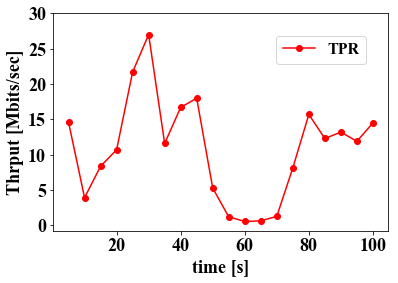
\includegraphics[width=70mm,bb=9 9 358 434]{image/Thrput.png}
        \caption{Throughput in a Cafe}
        \label{thrput}
    \end{center}
\end{figure}

Although the previous scheme is successful in the detection for hardware-based RAP in the experimental environment, it cannot detect accurately in the real world.
This is because throughput is considerably dependent on various factors of the network environment such as mobility of the traffic, collisions, network topology changes, and unintentional interference.
\figurename~\ref{thrput} is the graph which shows the change of throughput in a cafe on a weekday.
Since the traffic in real environment is unsteady as shown in \figurename~\ref{thrput} in fact, the previous scheme is subject to environmental changes, which can lead to degrade the accuracy.
Thus, the requirement that we must satisfy is to leverage factors which are independent of the network environment for the detection.

\section{PROPOSED SCHEME}\label{sec:4}
In order to meet the requirements mentioned in Section \ref{sec:shortcoming}, in this paper, we propose \title{}.
In the following subsections, we firstly explain the idea of the proposed scheme.
In the next subsection, the algorithm is described in detail.

\subsection{Idea}
The main idea of the proposed scheme is that there exist two APs, namely, the RAP and a LAP, on the same path from a user device to a gateway.
In general, a LAP is the only device which exists on the path.
Therefore, in this case, the LAP is identical to the AP directly connected with a user device.
In an attack scenario, besides the connected RAP, a LAP exists inevitably on the other side of the RAP due to a man-in-the-middle-attack.
Therefore, a connected AP can be revealed as the RAP when the presence of a LAP is detected on the same path.

On the basis of this idea, the proposed scheme reveals that a LAP is on the other side of the connected RAP by finding out the MAC address of a LAP.
In order to discover the MAC address of a LAP on the same path, we leverage the phenomenon that a user device cannot receive Address Resolution Protocol (ARP) reply packets in the situation where there exist duplicate MAC addresses on the same path.
The proposed scheme intentionally creates such situation by setting the MAC address of a user device to the MAC addresses obtained from beacon frames of APs in the communication range of a user device.
Note that the MAC address of the AP with which a user device connects is excluded from targets for setting MAC addresses.
If the MAC address of a user device is set to that of a LAP on the same path, a LAP receives ARP reply packets whose original destination is a user device before a user device receives them.
Thus, since a user device cannot receive ARP reply packets, it continues to resend ARP requests, which results in disabling internet connectivity.
By observing the continuance of resending ARP request packets within a definite period of time without ARP reply packets, the proposed scheme can reveal that there exists the RAP and a LAP on the path, which detects the attack.

When a user device connects with the RAP, there exists the MAC address of a LAP in the communication range of a user device.
This is because the RAP are located relatively near a LAP to avoid communication delay.
Hence, we can inevitably obtain the MAC address of a LAP in the case where there exists the RAP in a network.
In the real situation, it is possible that there exist several LAPs in a communication range of a user device.
Thus, we collect the only MAC addresses of APs which have the identical SSID to that of AP connected by a user device.
This is because RAP must utilize an SSID of a LAP for pretending to be LAP.
A user device can receive ARP reply packets even if its MAC address is set to that of each LAP on distinct paths.
This is because the MAC addresses can be duplicated except those on the same path.

Since the proposed scheme is independent of the real network environment, it is useful for overcoming the shortcoming of the previous scheme.
In addition to that, the proposed scheme is not affected by a spoofed MAC address because it focuses on the only legitimate MAC address never spoofed.

\subsection{Algorithm}
In this subsection, the algorithm for detection based on searching the MAC address of a LAP on the same path is explained.
The proposed algorithm mainly consists of 1) MAC address collection phase and 2) ARP reply based detection phase. 

\subsubsection{MAC Address Collection}
Let $\tarAP$ denote a AP which connects with a user's device.
The set of MAC addresses of APs whose SSIDs are identical to that of $\tarMAC$  in the communication range of a user's device is created through beacon frames of them. 
Let the set denote $M_{all}=\{M_{input}|0\le input \le n_{all}  \}$, where $n_{all}$ is the number of collected MAC addresses.

\subsubsection{ARP Reply based Detection}
\figurename~\ref{fig:flowchart} shows the flowchart of this phase.
As shown in \figurename~\ref{fig:flowchart}, this phase consists of four procedures which are 1) Comparison with $\tarMAC$, 2)Setting $\userMAC$ to \newcommand{\inputMAC}{M_{A_{input}}}$\inputMAC$ , 3) Observation of ARP reply from the gateway to the user device.
These procedures are repeatedly conducted for every $M_input$ in $M_{all}$ unless the RAP is detected.

In the first phase, the $\inputMAC$ and the $\tarMAC$ are compared.
If they are the same MAC address, it easily judges the either of them is the RAP due to the cloned address.
In this case, since RAP is detected, the detection phase is finished.
However, in the case where the RAP clones a MAC address of a LAP beyond the communication range of a user's device or it does not clone, the accordance of MAC addresses cannot be detected only by this MAC address checking.
Thus, the detection process goes to the second phase.

In the second phase, $\userMAC$ which denotes the MAC address of a user' s device is set to $\inputMAC$.

After $\userMAC$ is set to $\inputMAC$, the connection between the user device and $\tarAP$ is once lost since the gateway become unable to use the original MAC address as a destination for the packets.
Thus, the user device sends ARP request in order to reconnect with it through the $\tarAP$ automatically due to the stronger RSSI than any other $M_{all}$.

Finally, in the third procedure, the ARP reply packets whose destination is set as $\inputMAC$ are observed to investigate whether the $\inputAP$ is on the same path with the user's device.
If the packets do not reach the user's device, the $\tarAP$ can be revealed as the MAC address of the RAP which exists between the user device and the LAP with  $\inputAP$, and the detection phase is finished.
Otherwise, the $\tarAP$ is judged that it is on the distinct path from the $\inputAP$.
In this case, the same procedures in the flowchart are repeatedly conducted for another $\inputAP$ in $M_{A_{all}}$ until the RAP is detected.
If the detection phase is carried out for all $\inputAP$ without the detection of RAP, the $\tarAP$ is declared as a LAP. 
%ARP is a procedure always done at the beginning of the Wi-Fi communication for mapping IP address to MAC address in a LAN to establish communication to the Internet and composed of two phases: ARP request, and ARP reply.
%ARP request is a packet sent by a user device to a gateway i.e. router of the LAN at the beginning of the network communication.
%Since MAC address is used for a destination address of a packet in LAN communication, the device cannnot communicate with the Internet, or even gateway, without the MAC address of the gateway.
%In order to acquire a MAC address of a gateway, ARP request packets, which includes source MAC address information, are sent to the gateway's IP address. 
%After the gateway get the packet from the device, ARP reply packets are sent by the gateway to the source device on the basis of the source MAC address included in ARP request packets, which can tell the gateway's MAC address by including it as a source MAC address.

\section{EVALUATION}\label{sec:5}
In order to demonstrate the effectiveness of the proposed scheme, we compare it with the scheme \cite{previous} which interferes the channel between a LAP and RAP explained above as a previous scheme.

The metric of the evaluations are Accuracy (ACC), TPR (True Positive Rate), and FPR (False Positive Rate) defined as
\begin{gather}
    ACC = \frac{TP + TN}{TP + TN + FP + FN} \\
    TPR = \frac{TP}{TP + FN} \\
    FPR = \frac{FP}{FP + TN}
\end{gather}
where TP, TN, FP, and FN denote the number of True Positive (RAPs is reregarded as RAPs), True Negative (LAPs are regarded as LAPs), False Positive (LAPs are regarded as RAPs), and False Negative (RAPs are regarded as LAPs), respectively.
We evaluate our scheme with these metrics by two scenarios which are the case of attack where a user device connects with a RAP and that of non-attack where a user device connects with a LAP.

\subsection{Experimental Setup}
We implemented the detectors in a laptop, which is a MacBook Pro with an Intel Core i5 CPU and 16GB RAM.
In order to configure \cite{previous} for comparison, we use a TP-Link Archer C6 as an interference device.

Simiraly, the same AP devices are used for both LAP and RAP.
In additon, in order to set a RAP up for distinct channel from a LAP, TP-Link Archer C50 is introduced as a repeater between the RAP and the LAP.
These two APs, where one is in the station mode and the other is in AP mode, are interconnected using a LAN cable.
All devices are operated in the IEEE 802.11n mode with MIMO.
We arrange a LAP, RAP, and user device at equal intervals and it is about 5 feet.

\subsection{Traffic Scenario}
In order to demonstrate the robustness against unstable traffic in real environment, we intentionally generate random traffic to the LAP at random time in each experiment.

\subsection{Time of Detection}
The experiments are conducted for each case, namely attack scenario and non attack scenario 100 times.
The average time required per detection is represented as $T$.
It is affected by the observation time of ARP procedure per AP, which is represented as $\Delta t$ , and also the number of LAPs before a RAP is detected in an attack scenario.
We conduct each evaluation by changing $\Delta t$ from 5 seconds to 10 seconds at every second.

\subsection{Evaluation of the Proposed Scheme}

\begin{figure}[t]
    \begin{minipage}{0.33\hsize}
        \begin{center}
            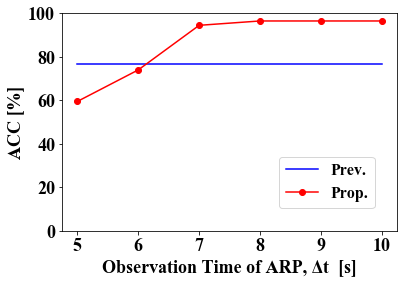
\includegraphics[width=20mm,bb=9 9 358 434]{image/ACC.png}
        \end{center}
        \caption{The ACC of the Proposed Scheme}
        \label{fig:acc}
    \end{minipage}
    \begin{minipage}{0.33\hsize}
        \begin{center}
            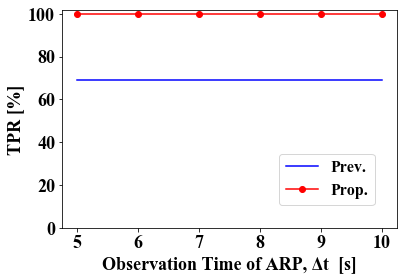
\includegraphics[width=20mm,bb=9 9 358 434]{image/TPR.png}
        \end{center}
        \caption{The TPR of the Proposed Scheme}
        \label{fig:tpr}
    \end{minipage}
    \begin{minipage}{0.33\hsize}
        \begin{center}
            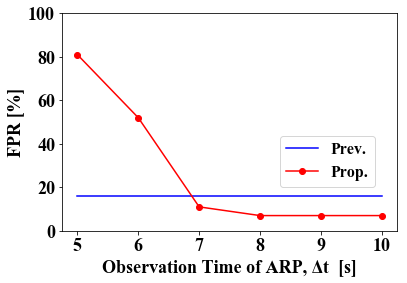
\includegraphics[width=20mm,bb=9 9 358 434]{image/FPR.png}
        \end{center}
        \caption{The FPR of the Proposed Scheme}
        \label{fig:fpr}
    \end{minipage}

\end{figure}
First, in order to show the effectiveness of the proposed scheme (Prop.), we compare it with the previous scheme \cite{previous} (Prev.).
\figurename~\ref{fig:acc}, \ref{fig:tpr}, and\ref{fig:fpr} show the results of our evaluations for each scheme.
The both schemes are conducted in the random traffic scenario.
As shown in \figurename~\ref{fig:acc}, the previous scheme cannot accurately detect the attack, and the ACC is about 69\%.
As regards the proposal scheme, however the ACC is lower than that of \cite{previous} when each ARP observation time is not greater than 6s, it is getting higher with the observation time.
In particular, in the case where the time is longer than 7s, ACC is improved up to 96.5\% in the propsed scheme.

As a result, shown in \figurename~\ref{fpr}, the longer each observation time is, the lower FPR is in the proposal scheme.
It improves up to 74\% in the result of the last three time settings compared with that of the beginning.
In additon, as shown in \figurename~\ref{tpr}, TPR of the proposed scheme is 100.0\% regardless of the observation time, which means it never pass a RAP over in an attack scenario.

In order to reveal the reason of these results, we analyze the ARP packets in detail.
Through the packet analysis, we disclose the reason is that the time for finishing ARP procedure tends to be longer than 6s and it is not always fixed.
Thus, in the case of less than 7.0 seconds, several LAPs are detected as RAPs incorrectly since it is not enough for a user device to get ARP reply packets while the reverse is never happen.
Given the fact, we conduct the further experiment to realize more precise detection by setting enough time to auquire ARP reply packets.
As a result, we conclude that the proposed scheme enables the detection without any error when the $\Delta t$ is set to 15 seconds.

\subsection{Evaluation in a Real Environment}
In order to demonstrate the robustness and reruired time of the proposed scheme in a real environment, we conduct an experiment in a cafe and evaluate ACC and the total time required for the detection.
There exists three APs arranged, whose SSID are all same.
In the attack scenario, one of them is replaced by a RAP, which has a same SSID.
In the same way with the experiment in the previous subsection, we conduct the proposed scheme in the both cases where a user's device connects with a RAP or a LAP.
The experiments are conducted around 2:00pm on a weekday at an cafe.
The observation time of ARP procedure is set to 15 seconds enough to get ARP reply packets.
\tablename~\ref{tab:real} shows the results in the real environment.
Our scheme realize 100\% accuracy even in a real environment if the time for observation of ARP procedure is enough.
At that time, the average total time per detection is 32.1 seconds.

\begin{table}[htb] 
    \begin{center}
        \caption{Evaluation Result in Real Environment}
        \begin{tabular}{c c} \hline
            ACC (\%) & Avg. Total Time (s) \\ \hline \hline
            100.0 & 32.1 \\ \hline
        \end{tabular}
    \end{center}
\end{table}

Through this result, we conclude that the proposed proposal can accurately detect the attack even in a real environment whose traffic is unstable.
However, as with other existing schemes, the proposed scheme also assumes Wi-Fi network models where legitimate repeaters are not installed.
It may be usual to introduce a legitimate repeater in their network to relay traffic farther at the expense of transmission speed in a large area.
In this case, the proposed scheme cannot distinguish a RAP and legitimate repeater since both of them relay packets between a user device and a LAP in the same way as man-in-the-middle.
However, in order to detect the attack even in such Wi-Fi networks, we focus on their RSSI values.
Since a legitimate repeater has a function to rely packets from a LAP to devices which cannot connect with the LAP due to the long distance, it should be located far from a LAP in general.
In contrast, a RAP is basically introduced near a connecting LAP not to cause traffic delay due to their long distance.
Thus, we assume that a AP can be judged whether it is a legitimate repeater or not on the basis of this idea.
In the future, we plan to devise the additional countermeasures and conduct experiments so as to distinguish legitimate repeater with RSSI value, which can tell their general distance each other \cite{rssi}.

\section{conclusion}\label{sec:6}
\begin{thebibliography}{00}
\bibitem{snooping1} A. Adya, P. Bahl, R. Chandra, and L. Qiu, “Architecture and techniques for diagnosing faults in IEEE 802.11 infrastructure networks,”n Proc. of ACM Annual International Co.nference on Mobile Computing and Networking, MOBICOM, 2004, pp. 30-44.
\bibitem{snooping2} P. Bahl, R. Chandra, J. Padhye, L. Ravindranath, M. Singh, A. Wolman, and B. Zill, “Enhancing the security of corporate Wi-Fi etworks using DAIR,” in Proc. of ACM International Conference on Mobile Systems, Applications, and Services, MobiSys, 2006, pp. 1–14.
\bibitem{snooping3} R. Chandra, J. Padhye, A. Wolman, and B. Zill, “A location-based management system for enterprise wireless LANs,” in Proc. of USENIX Symposium on Networked Systems Design and Implementation NSDI, 2007.
\bibitem{rssi1} D. B. Faria and D. R. Cheriton, “Detecting identity-based attacks in wireless networks using signalprints,” in Proc. of ACM Workshop on Wireless Security, 2006, pp. 43–52.
\bibitem{rssi2} Y. Sheng, K. Tan, G. Chen, D. Kotz, and A. Campbell, “Detecting 802.11 MAC layer spoofing using received signal strength,” in Proc. of the 27th Conference on Computer Communications, INFOCOM, 2008.
\bibitem{clock1} F. Lanze, A. Panchenko, B. Braatz, and T. Engel, “Letting the puss in boots sweat: detecting fake access points using dependency of clock skews on temperature,” in Proc. of ACM Symposium on Information, Computer and Communications Security, ASIACCS, 2014, pp. 3–14.
\bibitem{clock2} S. Jana and S. K. Kasera, “On fast and accurate detection of unauthorized wireless access points using clock skews,” IEEE Trans. Mob. Comput., vol. 9, no. 3, pp. 449–462, 2010.
\bibitem{channel1} V. Brik, S. Banerjee, M. Gruteser, and S. Oh, “Wireless device identifica- tion with radiometric signatures,” in Proc. ofACM Annual International Conference on Mobile Computing and Networking, MOBICOM, 2008.
\bibitem{traceroute} S. Nikbakhsh, A. B. A. Manaf, M. Zamani, and M. Janbeglou, “A novel approach for rogue access point detection on the client-side,” 27th International Conference on Advanced Information Networking and Applications Workshops, 2012.
\bibitem{rtt} H. Han, B. Sheng, C. C. Tan, Q. Li, and S. Lu, “A timing-based scheme for rogue AP detection,” IEEE Trans. Parallel Distrib. Syst., vol. 22, no. 11, pp. 1912–1925, 2011
\bibitem{iat} C. Yang, Y. Song, and G. Gu, “Active user-side evil twin access point detection using statistical techniques,” IEEE Trans. Information Forensics and Security, vol. 7, no. 5, pp. 1638–1651, 2012.
\bibitem{previous} R. Jang, J. Kang, A. Mohaisen and D. Nyang, "Catch Me If You Can: Rogue Access Point Detection Using Intentional Channel Interference," in IEEE Transactions on Mobile Computing.

\end{thebibliography}
\vspace{12pt}
\end{document}
